\documentclass[12pt,a4paper]{article}

% ------------------------------------------------------------
% Encoding, language, fonts
% ------------------------------------------------------------
\usepackage[T1]{fontenc}
\usepackage[utf8]{inputenc}
\usepackage[english]{babel}
\usepackage{lmodern}
\usepackage{microtype}

% ------------------------------------------------------------
% Page layout
% ------------------------------------------------------------
\usepackage{pdflscape}

% ------------------------------------------------------------
% Mathematics, tables, figures
% ------------------------------------------------------------
\usepackage{amsmath,amssymb,amsfonts,amsthm}
\usepackage{mathtools}
\usepackage{array,booktabs}
\usepackage{float}
\usepackage{graphicx}

% ------------------------------------------------------------
% Plots
% ------------------------------------------------------------
\usepackage{pgfplots}
\pgfplotsset{compat=1.17}

% ------------------------------------------------------------
% Bibliography
% Compile with: pdfLaTeX -> Biber -> pdfLaTeX -> pdfLaTeX
% ------------------------------------------------------------
\usepackage{csquotes}
\usepackage[backend=biber,style=numeric,sorting=none]{biblatex}
\addbibresource{references.bib}

% ------------------------------------------------------------
% Code listings for Python and VBA attachments
% ------------------------------------------------------------
\usepackage{xcolor}
\usepackage{upquote}
\usepackage{listings}

\definecolor{codebackground}{RGB}{248,248,248}
\definecolor{codegray}{gray}{0.45}

\lstdefinestyle{commoncodestyle}{
    inputencoding=utf8,
    extendedchars=true,
    backgroundcolor=\color{codebackground},
    basicstyle=\ttfamily\tiny,
    keywordstyle=\bfseries\color{blue!60!black},
    commentstyle=\itshape\color{green!40!black},
    stringstyle=\color{red!55!black},
    numbers=left,
    numberstyle=\tiny\color{codegray},
    stepnumber=1,
    numbersep=5pt,
    frame=single,
    framerule=0.3pt,
    framesep=3pt,
    rulecolor=\color{black!30},
    breaklines=true,
    breakatwhitespace=false,
    breakindent=1em,
    breakautoindent=true,
    postbreak=\mbox{\textcolor{codegray}{$\hookrightarrow$}\space},
    showstringspaces=false,
    columns=flexible,
    keepspaces=true,
    tabsize=4,
    captionpos=t,
    upquote=true,
    linewidth=\linewidth,
    xleftmargin=0pt,
    xrightmargin=0pt,
    literate={é}{{\'e}}1 {É}{{\'E}}1 {ä}{{\"a}}1 {ö}{{\"o}}1 {ü}{{\"u}}1 {Ä}{{\"A}}1 {Ö}{{\"O}}1 {Ü}{{\"U}}1 {ß}{{\ss}}1 {–}{{--}}1 {—}{{---}}1 {’}{{'}}1 {‘}{{'}}1 {“}{{``}}1 {”}{{''}}1 {≤}{{$\leq$}}1 {≥}{{$\geq$}}1 {→}{{$\to$}}1
}

\lstdefinestyle{pythonstyle}{
    style=commoncodestyle,
    language=Python
}

\lstdefinelanguage{VBA}{
    morekeywords={
        Option, Explicit, Public, Private, Sub, Function, End, If, Then, Else,
        ElseIf, For, To, Step, Next, Each, In, Do, While, Loop, Dim, As, Set,
        Const, ByRef, ByVal, Optional, Call, Exit, ReDim, With, True, False,
        Nothing, And, Or, Not, Mod, Select, Case, On, Error, Resume, GoTo,
        Worksheet, ChartObject, Long, Double, String, Boolean, Variant
    },
    sensitive=false,
    morecomment=[l]{'},
    morestring=[b]"
}

\lstdefinestyle{vbastyle}{
    style=commoncodestyle,
    language=VBA
}

\renewcommand{\lstlistingname}{Listing}
\renewcommand{\lstlistlistingname}{List of Listings}

% ------------------------------------------------------------
% Names of lists
% ------------------------------------------------------------
\renewcommand{\contentsname}{Contents}
\renewcommand{\listfigurename}{List of Figures}
\renewcommand{\listtablename}{List of Tables}

\renewcommand{\lstlistingname}{Code Listing}
\renewcommand{\lstlistlistingname}{List of Code Listings}
% ------------------------------------------------------------
% Short code snippets inside the main text
% -------------------------------------------------
\lstdefinestyle{pythontextstyle}{
    style=pythonstyle,
    basicstyle=\ttfamily\footnotesize,
    numbers=none,
    frame=single,
    framerule=0.3pt,
    breaklines=true,
    breakatwhitespace=false,
    captionpos=t
}

\lstdefinestyle{vbatextstyle}{
    style=vbastyle,
    basicstyle=\ttfamily\footnotesize,
    numbers=none,
    frame=single,
    framerule=0.3pt,
    breaklines=true,
    breakatwhitespace=false,
    captionpos=t
}
% ------------------------------------------------------------
% Hyperlinks
% Hyperref should be loaded near the end of the preamble.
% ------------------------------------------------------------
\usepackage[hidelinks]{hyperref}

% ------------------------------------------------------------
% Layout safety for long expressions and URLs
% ------------------------------------------------------------
\emergencystretch=3em
\setlength{\parindent}{0pt}
\setlength{\parskip}{0.8em}
% ------------------------------------------------------------
% Document begins
% ------------------------------------------------------------
\begin{document}
\pagenumbering{gobble}

% ------------------------------------------------------------
% Title page
% ------------------------------------------------------------
\begin{titlepage}
    \centering

    \begin{flushright}
        
\includegraphics[width=0.5\linewidth]{Logo-Hochschule-Darmstadt.png}
    \end{flushright}

    \vspace{1.5cm}

    \textbf{\large Seminar paper in the field of Mathematics and Natural Sciences\\
    Bachelor's program in Applied Mathematics}

    \vspace{1.5cm}

    {\huge\bfseries Mean-Preserving B\'ezier Interpolation of Hydrochemical Time-Series Data under Physical Constraints\par}

    \vspace{2cm}

    {\Large Yana Osinchuk\par}

    \vspace{1cm}

    {\Large May 20, 2026\par}

    \vfill

    \begin{flushleft}
        The topic presented \hfill Second examiner\\
        Prof.\ Dr.\ Thomas Maerz \hfill All present\\
    \end{flushleft}
\end{titlepage}
\pagenumbering{roman}

% ------------------------------------------------------------
% Declaration
% ------------------------------------------------------------
\newpage
\section*{Declaration}
\addcontentsline{toc}{section}{Declaration}

I affirm that I have independently authored this seminar document and have not used sources or aids other than those explicitly mentioned. Any directly quoted or paraphrased passages from other works are appropriately acknowledged.
\\
\\
\\
\\Osinchuk Yana

% ------------------------------------------------------------
% Summary
% ------------------------------------------------------------
\newpage
\section*{Summary}
\addcontentsline{toc}{section}{Summary}

This study examines B\'ezier-based interpolation methods for the approximation of hydrochemical and hydrological time-series data subject to simultaneous mathematical and physical constraints. The main objective is to construct an interpolatory framework capable of producing a smooth representation of the measured process while satisfying prescribed endpoint, integral, and shape conditions. In particular, on each interpolation interval, the constructed curve is required to pass through the initial and terminal data values, preserve the prescribed interval mean, incorporate derivative information when available, and remain within physically admissible bounds.
\\
\\Conventional interpolation schemes can generate smooth approximating curves; however, they do not, in general, guarantee the preservation of integral characteristics such as interval mean values. Moreover, standard interpolation methods may produce overshoots or undershoots that are inconsistent with the physical nature of hydrological and hydrochemical variables. To overcome these limitations, several modified B\'ezier formulations are developed and compared. The considered methods include a mean-preserving cubic B\'ezier construction, an exact quartic B\'ezier formulation with derivative constraints, and a modified bounded quartic B\'ezier formulation with soft derivative constraints. In the latter method, derivative estimates are treated as reference slopes rather than as unconditional constraints. The algorithms were first implemented and tested in Python, where numerical experiments and graphical diagnostics were performed, and were subsequently translated into Excel through Visual Basic for Applications (VBA) to enable their use within a spreadsheet-based operational workflow.
\\
\\The performance of the proposed methods is assessed through visual comparison with the measured data and quantitative error analysis. The evaluation is based on standard statistical metrics, including the root-mean-square error \(\mathrm{RMSE}\), the mean absolute error \(\mathrm{MAE}\), the maximum absolute error, and the coefficient of determination \(R^2\). The comparison is designed to assess not only approximation accuracy, but also the preservation of endpoint values, interval means, derivative behavior, and physical bounds.

\newpage
\begin{otherlanguage}{ngerman}
\section*{Zusammenfassung}
\addcontentsline{toc}{section}{Zusammenfassung}

Diese Arbeit untersucht B\'ezier-basierte Interpolationsmethoden zur Approximation hydrochemischer und hydrologischer Zeitreihendaten unter gleichzeitiger Ber\"ucksichtigung mathematischer und physikalischer Nebenbedingungen. Das Hauptziel besteht darin, ein Interpolationsverfahren zu konstruieren, das eine glatte Darstellung des gemessenen Prozesses erzeugt und dabei vorgegebene Endpunkt-, Integral- und Formbedingungen erf\"ullt. Insbesondere soll die konstruierte Kurve auf jedem Interpolationsintervall durch die Anfangs- und Endwerte verlaufen, den vorgeschriebenen Intervallmittelwert erhalten, vorhandene Ableitungsinformationen einbeziehen und innerhalb physikalisch zul\"assiger Grenzen bleiben.

Konventionelle Interpolationsverfahren k\"onnen glatte approximierende Kurven erzeugen; im Allgemeinen garantieren sie jedoch nicht die Erhaltung integraler Eigenschaften, wie etwa von Intervallmittelwerten. Dar\"uber hinaus k\"onnen Standardverfahren \"Uber- oder Unterschwingungen erzeugen, die mit der physikalischen Bedeutung hydrologischer und hydrochemischer Gr\"o\ss en nicht vereinbar sind. Um diese Einschr\"ankungen zu \"uberwinden, werden mehrere modifizierte B\'ezier-Formulierungen entwickelt und verglichen. Die betrachteten Methoden umfassen eine mittelwerterhaltende kubische B\'ezier-Konstruktion, eine exakte quartische B\'ezier-Formulierung mit Ableitungsbedingungen sowie eine modifizierte beschr\"ankte quartische B\'ezier-Formulierung mit weichen Ableitungsbedingungen. Bei der letztgenannten Methode werden die Ableitungssch\"atzungen als Referenzsteigungen und nicht als uneingeschr\"ankte Nebenbedingungen behandelt. Die Algorithmen wurden zun\"achst in Python implementiert und getestet, wobei numerische Experimente und graphische Diagnosen durchgef\"uhrt wurden. Anschlie\ss end wurden sie in Excel mittels Visual Basic for Applications (VBA) \"ubertragen, um ihre Anwendung in einem tabellenbasierten Arbeitsablauf zu erm\"oglichen.

Die Leistungsf\"ahigkeit der vorgeschlagenen Methoden wird durch einen visuellen Vergleich mit den gemessenen Daten sowie durch eine quantitative Fehleranalyse bewertet. Die Auswertung basiert auf Standardmetriken, darunter die Wurzel des mittleren quadratischen Fehlers \(\mathrm{RMSE}\), der mittlere absolute Fehler \(\mathrm{MAE}\), der maximale absolute Fehler und das Bestimmtheitsma\ss{} \(R^2\). Der Vergleich ist darauf ausgelegt, nicht nur die Approximationsgenauigkeit, sondern auch die Erhaltung der Endpunktwerte, der Intervallmittelwerte, das Verhalten der Ableitungen und die Einhaltung physikalischer Grenzen zu beurteilen. Insbesondere wird erwartet, dass die beschr\"ankte quartische B\'ezier-Formulierung die physikalisch konsistenteste Darstellung liefert, da sie Mittelwerterhaltung mit ableitungsbasierter Formkontrolle und expliziten Zul\"assigkeitspr\"ufungen verbindet.

\end{otherlanguage}

% ------------------------------------------------------------
% Preface
% ------------------------------------------------------------
\newpage
\section*{Preface}
\addcontentsline{toc}{section}{Preface}

This research was completed under the supervision of Prof.\ Dr.\ Thomas Maerz, to whom I would like to express my sincere and profound gratitude. His continuous support, thoughtful guidance, and steady encouragement were invaluable throughout the development of this work.
\\
\\I am especially grateful for his willingness to discuss every difficulty in detail, for his clear and insightful explanations, and for the constructive feedback that accompanied this project from its initial ideas to its final implementation. His guidance not only strengthened my understanding of the interpolation methods investigated in this work, but also helped me translate the theoretical concepts into practical computational tools using Python and Excel.
\\
\\Sincere appreciation is also expressed to Mr.\ Andreas Burmeister from the Hessian Agency for Nature Conservation, Environment and Geology. His practical expertise, valuable suggestions, and experience with real environmental data added an important applied dimension to this work. Specifically, his openness in sharing his professional perspective was instrumental in relating the mathematical methods studied herein to concrete questions arising in hydrological and hydrochemical data analysis.

% ------------------------------------------------------------
% Contents
% ------------------------------------------------------------
% ------------------------------------------------------------
% Contents and lists
% ------------------------------------------------------------
\newpage
\tableofcontents

% ------------------------------------------------------------
% Introduction
% ------------------------------------------------------------
\newpage
\pagenumbering{arabic}

\section{Introduction}
Hydrochemical and hydrological monitoring frequently results in limited time series data, as the laboratory analysis of chemical elements and water quality parameters can often be expensive, time-consuming, or experimentally challenging. In environmental applications, sparse observations are commonly combined with interpolation or approximation procedures in order to support further analysis, modelling, visualization, and decision making \cite{gnauck2004waterquality,lepot2017interpolation,kokhan2013geoinformation}. The available observations therefore describe the underlying process only at discrete sampling times, whereas many subsequent tasks, including visualization, comparison of data sets, numerical integration, gap filling, trend detection, and model coupling, require a representation on a finer temporal scale \cite{gnauck2004waterquality,lepot2017interpolation}.

The choice of an interpolation or model-construction method is not merely a technical detail. In environmental and geospatial modelling, different interpolation methods may lead to different derived quantities and therefore affect subsequent calculations. For example, studies on digital elevation models and soil erosion show that the method used to construct an intermediate numerical surface can influence the results of later environmental computations \cite{piatkova2019dem}. This motivates the use of interpolation methods that are not only accurate, but also consistent with physical and statistical properties of the measured data.

In this paper, interpolation is treated as a constrained reconstruction problem rather than as a purely graphical smoothing procedure. On each interval, the interpolant should reproduce the measured endpoint values, preserve the prescribed interval mean, respect physically admissible bounds, and incorporate derivative information only when it is compatible with these restrictions. This viewpoint is related to classical interpolation and approximation of tabular data \cite{krylyk2013computational,deboor1978splines}, as well as to shape-preserving polynomial interpolation, where slopes or control parameters are restricted in order to avoid artificial extrema, loss of monotonicity, or violation of positivity \cite{fritsch1980monotone,fritsch1984monotone,scipyPchip}.

The chosen framework is based on B\'ezier polynomials. B\'ezier curves provide local geometric control through their control points: they interpolate the first and last control points, allow endpoint derivative information to be represented algebraically, and remain within the convex hull of the control polygon \cite{farin2002curves,piegl1997nurbs,mitBezierProperties,aaltoBezier2013}. These properties are particularly useful for hydrochemical data, since a visually smooth curve may still be physically inappropriate if it overshoots feasible concentration ranges or changes the average value represented by the measurements \cite{kokhan2013geoinformation,piatkova2019dem}. B\'ezier curves and Bernstein polynomials are classical tools in computer-aided geometric design and curve representation \cite{farin2002curves,piegl1997nurbs,pomaxBezierPrimer}.

Three B\'ezier-based constructions are investigated. First, a mean-preserving cubic segment is derived by selecting the inner control points so that the interval average is conserved. Second, an exact quartic B\'ezier formulation is used as a reference and diagnostic model, in which endpoint derivatives and interval means are imposed simultaneously. Third, a bounded quartic formulation is proposed, in which derivative estimates are treated as reference slopes: they are retained if they are compatible with the physical bounds and otherwise modified through projection onto the feasible set. The distinction between hard and soft derivative constraints follows the general idea of shape-preserving interpolation, where local derivative information is useful but must be controlled when it conflicts with admissibility \cite{fritsch1980monotone,fritsch1984monotone}.

The algorithms were first developed in Python for numerical experimentation, derivative estimation, graphical diagnostics, and error analysis. The final procedures were then implemented in Excel/VBA to make the methods usable in a spreadsheet-based workflow for hydrological and hydrochemical data. The paper is organized as follows: Section~2 recalls the required background on interpolation, B\'ezier curves, mean preservation, physical bounds, derivative estimation, and error metrics. Section~3 develops the mean-preserving cubic construction. Section~4 presents the quartic formulations, including the constrained method with soft derivative conditions. Section~5 describes the Python and Excel/VBA implementations. Section~6 discusses the numerical results and comparison of the methods. Section~7 summarizes the conclusions and possible extensions.

% ------------------------------------------------------------
% Main sections
% ------------------------------------------------------------
\newpage
\section{Theoretical Framework}

This section introduces the mathematical concepts and notation used throughout the paper. The aim is to define the interpolation problem, the prescribed constraints, the B\'ezier representation, and the quantitative criteria used to evaluate the resulting curves. The notation follows standard numerical analysis and geometric modelling literature on interpolation, piecewise polynomial curves, Bernstein polynomials, and B\'ezier representations \cite{krylyk2013computational,deboor1978splines,farin2002curves,piegl1997nurbs}.

\subsection{Discrete Time-Series Data and Support Points}

Let the measured data be given as a discrete time series
\[
(x_0^{\mathrm{ref}},y_0^{\mathrm{ref}}),
(x_1^{\mathrm{ref}},y_1^{\mathrm{ref}}),
\dots,
(x_N^{\mathrm{ref}},y_N^{\mathrm{ref}}),
\]
where \(x_j^{\mathrm{ref}}\) denotes time and \(y_j^{\mathrm{ref}}\) denotes the measured value of the hydrological or hydrochemical quantity considered. Discrete tabular data of this form are the standard starting point for interpolation and approximation problems \cite{krylyk2013computational,deboor1978splines}. It is assumed that the time values are strictly increasing,
\[
x_0^{\mathrm{ref}} < x_1^{\mathrm{ref}} < \dots < x_N^{\mathrm{ref}}.
\]
In practical applications, the complete measured data set may contain many values, while the interpolation method is constructed only on a smaller set of support points. These support points are denoted by
\[
(x_0,y_0),(x_1,y_1),\dots,(x_n,y_n),
\]
where
\[
x_0 < x_1 < \dots < x_n.
\]
The interval between two neighboring support points is written as
\[
I_i=[x_i,x_{i+1}],
\qquad i=0,\dots,n-1,
\]
and its length is
\[
h_i=x_{i+1}-x_i.
\]
The use of support points is closely connected to local piecewise interpolation: instead of constructing one global high-degree polynomial, the global curve is assembled from local segments, which improves stability and local control \cite{deboor1978splines,farin2002curves}.

\subsection{Interpolation and Approximation}

Interpolation is the construction of a function \(F\) that passes through prescribed data points. In the present setting, the interpolation condition is
\[
F(x_i)=y_i,
\qquad i=0,\dots,n.
\]
Since the curve is constructed locally on each interval \(I_i\), the interpolant can be written as a piecewise function
\[
F(x)=F_i(x),
\qquad x\in[x_i,x_{i+1}].
\]
Each local function \(F_i\) must satisfy the endpoint interpolation conditions
\[
F_i(x_i)=y_i,
\qquad
F_i(x_{i+1})=y_{i+1}.
\]
Classical numerical analysis distinguishes interpolation, where selected data values are reproduced exactly, from approximation, where the constructed function is evaluated by how well it represents a larger data set \cite{krylyk2013computational,deboor1978splines}. In this work both ideas are present. The constructed function interpolates the selected support points exactly, but it is also evaluated as an approximation of the full measured reference data. Similar interpolation and approximation ideas are frequently used in water-quality and environmental time-series analysis when data are available only at discrete measurement times \cite{gnauck2004waterquality,lepot2017interpolation}.

\subsection{Normalized Local Parameter}

For the construction of local B\'ezier curves, each interval \(I_i=[x_i,x_{i+1}]\) is mapped to the standard interval \([0,1]\). This normalization is standard in B\'ezier and spline curve representations, where polynomial segments are usually expressed in a local parameter rather than directly in the physical coordinate \cite{farin2002curves,piegl1997nurbs}. The normalized local parameter is defined by
\[
t=\frac{x-x_i}{h_i},
\qquad h_i=x_{i+1}-x_i.
\]
Thus,
\[
x=x_i+h_i t,
\qquad t\in[0,1].
\]
This transformation allows every local segment to be treated on the same parameter interval independently of its physical length. It also simplifies the formulas for B\'ezier control points, mean values, and endpoint derivatives \cite{farin2002curves,mitBezierProperties}.

\subsection{Interval Mean Constraint}

For each interval between two neighboring support points, a prescribed mean value is computed from the original reference measurements. Let \(s_i\) and \(e_i\) denote the indices of the first and last reference data points belonging to the interval \(I_i=[x_i,x_{i+1}]\). The prescribed empirical interval mean is defined by
\[
m_i=
\frac{1}{N_i}
\sum_{j=s_i}^{e_i}
y_j^{\mathrm{ref}},
\qquad
N_i=e_i-s_i+1.
\]
Thus, \(m_i\) is the arithmetic average of all measured reference values inside the interval, including both endpoints. This corresponds to the implementation in which all values between two consecutive support indices are summed and divided by the number of included values. Arithmetic averages of measured tabular values are commonly used as simple empirical representatives of interval behavior, especially when the data are sampled at a regular time step \cite{krylyk2013computational,gnauck2004waterquality}.

The interpolating curve is then required to preserve this empirical mean. For a local interpolating function \(F_i\) on the interval \(I_i=[x_i,x_{i+1}]\), the continuous mean value over this interval is defined by
\[
\frac{1}{h_i}
\int_{x_i}^{x_{i+1}} F_i(x)\,dx,
\qquad
h_i=x_{i+1}-x_i.
\]
Using the normalized local parameter, this expression can be rewritten as
\[
\frac{1}{h_i}
\int_{x_i}^{x_{i+1}} F_i(x)\,dx
=
\int_0^1 F_i(x_i+h_i t)\,dt.
\]
The mean-preserving condition therefore requires
\[
\int_0^1 F_i(x_i+h_i t)\,dt=m_i.
\]
In other words, the prescribed mean \(m_i\) is computed as an arithmetic average of discrete measured data, whereas the interpolating curve is required to have the same continuous average over the corresponding interval. This condition ensures that the interpolation not only matches endpoint values, but also preserves an integral characteristic of the original data. The importance of preserving physically meaningful averages is consistent with environmental modelling practice, where interpolation may influence later computations and interpretations \cite{kokhan2013geoinformation,piatkova2019dem}.

\subsection{Physical Bounds}

In hydrochemical and environmental applications, physical admissibility is as important as numerical smoothness, because interpolation may otherwise create values that have no meaningful interpretation. For example, water levels or concentrations should not become negative. More generally, one may require the interpolating curve to remain inside a physically admissible interval
\[
L\leq F_i(x)\leq U,
\qquad x\in I_i,
\]
where \(L\) is a lower bound and \(U\) is an optional upper bound \cite{kokhan2013geoinformation,gnauck2004waterquality}. If no upper bound is prescribed, one may formally set \(U=+\infty\).

In this work, physical admissibility is enforced through the control points of the B\'ezier curve. This gives a simple sufficient condition for boundedness: if all control points of a scalar B\'ezier segment lie inside the interval \([L,U]\), then the complete B\'ezier curve also lies inside \([L,U]\). This follows from the convex hull property of B\'ezier curves, which is a standard property derived from the non-negativity and partition-of-unity properties of the Bernstein basis \cite{farin2002curves,piegl1997nurbs,aaltoBezier2013,mitBezierProperties}.

\subsection{Bernstein Basis Polynomials}

The Bernstein basis polynomials of degree \(d\) are defined by
\[
b_{k,d}(t)=
\binom{d}{k}(1-t)^{d-k}t^k,
\qquad k=0,\dots,d,
\qquad t\in[0,1].
\]
The Bernstein basis is the classical polynomial basis used in B\'ezier curve representations \cite{farin2002curves,piegl1997nurbs,pomaxBezierPrimer}. The basis functions are non-negative on \([0,1]\),
\[
b_{k,d}(t)\geq 0,
\]
and form a partition of unity,
\[
\sum_{k=0}^{d} b_{k,d}(t)=1.
\]
These two properties imply that any B\'ezier curve is a convex combination of its control points for every \(t\in[0,1]\). This is the mathematical basis of the convex hull property used later to enforce physical bounds \cite{aaltoBezier2013,mitBezierProperties}.

\subsection{B\'ezier Curves}

A scalar B\'ezier curve of degree \(d\) with control points
\[
P_0,P_1,\dots,P_d
\]
is defined as
\[
B(t)=
\sum_{k=0}^{d} P_k b_{k,d}(t),
\qquad t\in[0,1].
\]
Equivalently,
\[
B(t)=
\sum_{k=0}^{d}
P_k
\binom{d}{k}
(1-t)^{d-k}t^k.
\]
This representation is standard in computer-aided geometric design and is valued because it combines polynomial simplicity with geometric control through the control polygon \cite{farin2002curves,piegl1997nurbs}. The first and last control points are exactly interpolated:
\[
B(0)=P_0,
\qquad
B(1)=P_d.
\]
Therefore, by choosing
\[
P_0=y_i,
\qquad
P_d=y_{i+1},
\]
one obtains a B\'ezier segment that passes through the endpoints of the interval \cite{mitBezierProperties,farin2002curves}.

The B\'ezier curve lies within the convex hull of its control points. In the scalar case, this means
\[
\min_{0\leq k\leq d} P_k
\leq
B(t)
\leq
\max_{0\leq k\leq d} P_k,
\qquad t\in[0,1].
\]
Consequently, if
\[
L\leq P_k\leq U
\qquad \text{for all } k,
\]
then
\[
L\leq B(t)\leq U
\qquad \text{for all } t\in[0,1].
\]
This property is one of the main reasons why B\'ezier curves are suitable for physically constrained interpolation \cite{farin2002curves,piegl1997nurbs,aaltoBezier2013}.

A further property that is essential for this work is the integral of a B\'ezier curve over the normalized interval. Since
\[
\int_0^1 b_{k,d}(t)\,dt=\frac{1}{d+1},
\]
it follows that
\[
\int_0^1 B(t)\,dt
=
\frac{1}{d+1}
\sum_{k=0}^{d} P_k.
\]
Therefore, the mean value of a B\'ezier curve over \([0,1]\) is equal to the arithmetic mean of its control points. This simple integral formula is a direct consequence of the Bernstein basis and is central to the mean-preserving construction used in this work \cite{farin2002curves,pomaxBezierPrimer}.

The derivative of a B\'ezier curve is again a B\'ezier curve of one degree lower. In particular,
\[
\frac{dB}{dt}(t)
=
d\sum_{k=0}^{d-1}(P_{k+1}-P_k)b_{k,d-1}(t).
\]
Thus, the endpoint derivatives with respect to the local parameter \(t\) are
\[
\frac{dB}{dt}(0)=d(P_1-P_0),
\qquad
\frac{dB}{dt}(1)=d(P_d-P_{d-1}).
\]
Because \(x=x_i+h_i t\), derivatives with respect to the original variable \(x\) satisfy
\[
\frac{dB}{dx}=\frac{1}{h_i}\frac{dB}{dt}.
\]
These derivative formulas allow endpoint derivative estimates to be translated directly into inner control points \cite{farin2002curves,piegl1997nurbs,mitBezierProperties}.

\subsection{Derivative Estimation}

In most practical data sets, derivative values are not measured directly. Therefore, they must be estimated from neighboring support points. The simplest estimate is based on secant slopes. On the interval \([x_i,x_{i+1}]\), the secant slope is
\[
\delta_i=
\frac{y_{i+1}-y_i}{x_{i+1}-x_i}
=
\frac{y_{i+1}-y_i}{h_i}.
\]
A basic finite-difference approximation for an interior derivative is
\[
d_i\approx
\frac{y_{i+1}-y_{i-1}}{x_{i+1}-x_{i-1}}.
\]
Finite differences are simple and widely used in numerical computation, but for irregular or noisy data they may produce large derivative values and may lead to overshoot. For this reason, shape-preserving derivative estimates are often preferable in interpolation problems \cite{deboor1978splines,fritsch1980monotone,fritsch1984monotone}.

In this work, a PCHIP-like derivative estimate is used. For an interior support point \(x_i\), let \(\delta_{i-1}\) and \(\delta_i\) be the neighboring secant slopes. If these slopes have opposite signs, or if one of them is zero, the derivative is set to zero:
\[
d_i=0
\qquad
\text{if}
\qquad
\delta_{i-1}\delta_i\leq 0.
\]
This prevents the introduction of artificial local extrema. If the two neighboring secant slopes have the same sign, the derivative is defined as a weighted harmonic mean,
\[
d_i=
\frac{w_1+w_2}
{\dfrac{w_1}{\delta_{i-1}}+\dfrac{w_2}{\delta_i}},
\]
where
\[
w_1=2h_i+h_{i-1},
\qquad
w_2=h_i+2h_{i-1}.
\]
This construction follows the idea of monotone piecewise cubic Hermite interpolation, where derivative values are selected locally to reduce overshoot and preserve the qualitative shape of the data \cite{fritsch1980monotone,fritsch1984monotone}. The SciPy implementation of \texttt{PchipInterpolator} is based on the same principle and documents its monotonicity-preserving and non-overshooting behavior for non-smooth data \cite{scipyPchip}.

\subsection{Error Metrics}

To evaluate the quality of the interpolation, the constructed curve is compared with the measured reference data. Let
\[
\widehat{y}_j=F(x_j^{\mathrm{ref}})
\]
be the interpolated value at the reference point \(x_j^{\mathrm{ref}}\). The residual is defined as
\[
e_j=y_j^{\mathrm{ref}}-\widehat{y}_j.
\]
Standard model-evaluation practice often uses several error measures simultaneously, because different metrics emphasize different properties of the residuals \cite{chai2014rmse,willmott2005mae}. The root-mean-square error is
\[
\mathrm{RMSE}=
\sqrt{
\frac{1}{N+1}
\sum_{j=0}^{N}e_j^2
}.
\]
The mean absolute error is
\[
\mathrm{MAE}=
\frac{1}{N+1}
\sum_{j=0}^{N}|e_j|.
\]
The maximum absolute error is
\[
E_{\max}=
\max_{0\leq j\leq N}|e_j|.
\]
The coefficient of determination is
\[
R^2=
1-
\frac{
\sum_{j=0}^{N}\left(y_j^{\mathrm{ref}}-\widehat{y}_j\right)^2
}{
\sum_{j=0}^{N}\left(y_j^{\mathrm{ref}}-\bar{y}^{\mathrm{ref}}\right)^2
},
\]
where
\[
\bar{y}^{\mathrm{ref}}=
\frac{1}{N+1}
\sum_{j=0}^{N}y_j^{\mathrm{ref}}.
\]
A smaller value of \(\mathrm{RMSE}\), \(\mathrm{MAE}\), or \(E_{\max}\) indicates a better approximation. A value of \(R^2\) close to \(1\) indicates that the interpolating curve explains most of the variation in the reference data. RMSE and MAE are both useful because RMSE penalizes large deviations more strongly, while MAE gives a more direct average absolute error \cite{chai2014rmse,willmott2005mae}.

\subsection{Roughness of the Control Polygon}

In addition to error metrics, it is useful to consider a simple measure of local roughness. Smoothness and local bending are classical concerns in spline and geometric curve design \cite{deboor1978splines,farin2002curves}. For a B\'ezier segment with control points \(P_0,\dots,P_d\), a discrete roughness indicator can be defined using second differences:
\[
\mathcal{R}_i=
\sum_{k=0}^{d-2}
\left(P_k-2P_{k+1}+P_{k+2}\right)^2.
\]
For the complete piecewise interpolant, the total roughness is
\[
\mathcal{R}=
\sum_{i=0}^{n-1}\mathcal{R}_i.
\]
This quantity is not an interpolation constraint. It is used only as a diagnostic indicator: large values of \(\mathcal{R}\) may indicate strong local bending or possible oscillatory behavior. The idea is consistent with the general use of derivative or curvature-related quantities to evaluate the regularity of piecewise polynomial curves \cite{deboor1978splines,farin2002curves}.

\subsection{Piecewise Continuity}

The global interpolant is constructed by joining local B\'ezier segments. Since the right endpoint of one segment and the left endpoint of the next segment are both equal to the same support value, the piecewise curve is continuous:
\[
F_i(x_{i+1})=y_{i+1}=F_{i+1}(x_{i+1}).
\]
Thus, \(F\in C^0\). Piecewise polynomial interpolation often distinguishes between continuity of function values and continuity of derivatives; this distinction is fundamental in spline theory and curve design \cite{deboor1978splines,farin2002curves}.

Higher-order smoothness, such as \(C^1\)-continuity, requires the derivatives of neighboring segments to match at the shared support point. If the same derivative estimate is used from both sides, derivative continuity can be encouraged. However, in the bounded method, derivative values may be adjusted in order to preserve physical admissibility. Therefore, exact \(C^1\)-continuity is not always imposed as a hard requirement. This trade-off between smoothness and shape preservation is consistent with the philosophy of monotone and shape-preserving interpolation \cite{fritsch1980monotone,fritsch1984monotone}.

\subsection{Summary of Required Constraints}

The interpolation methods considered in this work are designed to satisfy several conditions simultaneously. For each interval \(I_i=[x_i,x_{i+1}]\), the desired requirements are
\[
F_i(x_i)=y_i,
\qquad
F_i(x_{i+1})=y_{i+1},
\]
\[
\int_0^1 F_i(x_i+h_i t)\,dt=m_i,
\]
and
\[
L\leq F_i(x)\leq U,
\qquad x\in I_i.
\]
When derivative information is used, the reference derivative conditions are
\[
F_i'(x_i)\approx d_i,
\qquad
F_i'(x_{i+1})\approx d_{i+1}.
\]
In the exact quartic formulation, these derivative conditions are imposed as hard constraints. In the bounded quartic formulation, they are treated as soft reference conditions and are adjusted if necessary to preserve the physical bounds. This distinction combines ideas from B\'ezier curve control, convex-hull-based admissibility, and shape-preserving derivative estimation \cite{farin2002curves,piegl1997nurbs,fritsch1980monotone,fritsch1984monotone}.

\newpage
\section{Mean-Preserving Cubic B\'ezier Interpolation}

A cubic B\'ezier curve has degree \(3\) and four control points
\[
P_0,P_1,P_2,P_3.
\]
It is given by
\[
B(t)=(1-t)^3P_0+3(1-t)^2tP_1+3(1-t)t^2P_2+t^3P_3.
\]
The cubic B\'ezier curve is one of the most commonly used polynomial B\'ezier forms because it provides a useful balance between simplicity and shape control \cite{farin2002curves,piegl1997nurbs,pomaxBezierPrimer}. The endpoint interpolation conditions are
\[
B(0)=P_0,
\qquad
B(1)=P_3.
\]
For the interval \(I_i=[x_i,x_{i+1}]\), we set
\[
P_0=y_i,
\qquad
P_3=y_{i+1}.
\]
The mean value of the cubic B\'ezier segment is
\[
\int_0^1B(t)\,dt=
\frac{P_0+P_1+P_2+P_3}{4},
\]
which follows directly from the integral property of the Bernstein basis \cite{farin2002curves,aaltoBezier2013}. Therefore, the mean-preserving condition is
\[
\frac{P_0+P_1+P_2+P_3}{4}=m_i.
\]
Since \(P_0\) and \(P_3\) are fixed by the endpoint values, the two inner control points must satisfy
\[
P_1+P_2=4m_i-P_0-P_3.
\]
This shows that the cubic B\'ezier formulation has one remaining degree of freedom after the endpoint and mean conditions have been imposed. The situation is typical for constrained interpolation: after the required interpolation and mean constraints are imposed, an additional selection principle is needed to obtain a unique segment \cite{krylyk2013computational,deboor1978splines}.

To obtain a unique unconstrained cubic segment, the remaining degree of freedom can be fixed by choosing the smoothest segment in the sense of the second derivative. More precisely, the inner control points may be chosen to minimize
\[
J(P_1,P_2)=\int_0^1 \left(B''(t)\right)^2\,dt
\]
subject to the linear constraint
\[
P_1+P_2=4m_i-P_0-P_3.
\]
Second-derivative or curvature-related criteria are commonly used as smoothness indicators in spline and curve design \cite{deboor1978splines,farin2002curves}. This yields the preferred inner control points
\[
P_1^{\mathrm{pref}}=2m_i-\frac{1}{3}P_0-\frac{2}{3}P_3,
\qquad
P_2^{\mathrm{pref}}=2m_i-\frac{2}{3}P_0-\frac{1}{3}P_3.
\]
These formulas preserve constant data exactly: if \(P_0=P_3=m_i\), then \(P_1^{\mathrm{pref}}=P_2^{\mathrm{pref}}=m_i\).

If physical bounds are prescribed, the preferred pair \((P_1^{\mathrm{pref}},P_2^{\mathrm{pref}})\) is projected onto the feasible set determined by
\[
P_1+P_2=4m_i-P_0-P_3,
\qquad
L\leq P_1,P_2\leq U.
\]
This projection preserves the endpoint values and the interval mean exactly while ensuring that the B\'ezier segment remains inside the prescribed physical bounds whenever the feasible set is non-empty. The use of control-point bounds is justified by the convex hull property of B\'ezier curves \cite{farin2002curves,piegl1997nurbs,aaltoBezier2013}.

\newpage
\section{Quartic B\'ezier Interpolation with Derivative and Bound Constraints}

\subsection{Exact Quartic B\'ezier Formulation}

A quartic B\'ezier curve has degree \(4\) and five control points
\[
P_0,P_1,P_2,P_3,P_4.
\]
It is defined by
\[
B(t)=(1-t)^4P_0+4(1-t)^3tP_1+6(1-t)^2t^2P_2+4(1-t)t^3P_3+t^4P_4.
\]
Higher-degree B\'ezier curves provide additional degrees of freedom compared with cubic curves, but still preserve the same Bernstein basis structure and geometric interpretation \cite{farin2002curves,piegl1997nurbs}. The endpoint interpolation conditions are
\[
B(0)=P_0,
\qquad
B(1)=P_4.
\]
For the interval \(I_i=[x_i,x_{i+1}]\), we choose
\[
P_0=y_i,
\qquad
P_4=y_{i+1}.
\]
The mean value of the quartic B\'ezier segment is
\[
\int_0^1B(t)\,dt=
\frac{P_0+P_1+P_2+P_3+P_4}{5},
\]
again using the Bernstein integral formula \cite{farin2002curves,aaltoBezier2013}. Thus, the mean-preserving condition is
\[
\frac{P_0+P_1+P_2+P_3+P_4}{5}=m_i,
\]
or equivalently,
\[
P_1+P_2+P_3=5m_i-P_0-P_4.
\]

The endpoint derivatives with respect to \(x\) are
\[
B_x'(x_i)=\frac{4(P_1-P_0)}{h_i},
\qquad
B_x'(x_{i+1})=\frac{4(P_4-P_3)}{h_i}.
\]
These formulas follow from the derivative property of B\'ezier curves and the local parameter transformation \(x=x_i+h_i t\) \cite{farin2002curves,mitBezierProperties}. If derivative values \(d_i\) and \(d_{i+1}\) are imposed exactly, then
\[
P_1=P_0+\frac{h_i}{4}d_i,
\qquad
P_3=P_4-\frac{h_i}{4}d_{i+1}.
\]
The remaining middle control point is then determined by the mean condition:
\[
P_2=5m_i-P_0-P_1-P_3-P_4.
\]
Hence, a quartic B\'ezier curve has exactly enough degrees of freedom to satisfy five scalar conditions: two endpoint values, one interval mean, and two endpoint derivatives. However, if all these conditions are imposed exactly, the control points are uniquely determined. Consequently, physical bounds cannot always be satisfied simultaneously. This is analogous to other constrained interpolation settings, where imposing too many hard conditions may remove the degrees of freedom needed for shape preservation \cite{fritsch1980monotone,fritsch1984monotone}. For this reason, the exact quartic formulation is useful as a diagnostic reference, but it is not always physically admissible.

\subsection{Bounded Quartic B\'ezier Formulation with Soft Derivative Constraints}

In the bounded quartic method, the endpoint values and interval mean are kept as exact constraints, while the derivatives are treated as soft reference conditions. A derivative condition is called a hard constraint if it must be satisfied exactly. In the quartic B\'ezier case, the hard derivative constraints would be
\[
\frac{4(P_1-P_0)}{h_i}=d_i,
\qquad
\frac{4(P_4-P_3)}{h_i}=d_{i+1}.
\]
These equations uniquely determine \(P_1\) and \(P_3\). Together with endpoint interpolation and mean preservation, all five quartic control points are then fixed.

In contrast, a derivative condition is called a soft constraint if the derivative estimate is used only as a reference value. In this case, the derivative-based control points
\[
P_1^{\mathrm{ref}}=P_0+\frac{h_i}{4}d_i,
\qquad
P_3^{\mathrm{ref}}=P_4-\frac{h_i}{4}d_{i+1}
\]
are regarded as preferred values, but they may be adjusted if they would cause a violation of the physical bounds. This idea follows the same philosophy as shape-preserving interpolation: derivative information is useful for local shape control, but it must be limited when it creates nonphysical behavior or overshoot \cite{fritsch1980monotone,fritsch1984monotone,scipyPchip}. The resulting curve still preserves the endpoints and the interval mean exactly, but the endpoint derivatives are allowed to deviate from the reference slopes when necessary.

The bounded construction can be formulated as a projection problem. For the quartic case, define
\[
S_i=5m_i-P_0-P_4.
\]
The inner control points must satisfy
\[
P_1+P_2+P_3=S_i.
\]
Since
\[
P_2=S_i-P_1-P_3,
\]
it is sufficient to determine \(P_1\) and \(P_3\). The feasible set is
\[
\mathcal{C}_i=
\left\{(P_1,P_3):
L\leq P_1\leq U,
\;L\leq P_3\leq U,
\;L\leq S_i-P_1-P_3\leq U
\right\}.
\]
The bounded quartic construction chooses \(P_1\) and \(P_3\) as close as possible to the derivative-based reference values. This can be written as
\[
(P_1,P_3)=
\underset{(q_1,q_3)\in\mathcal{C}_i}{\operatorname{argmin}}
\left[
(q_1-P_1^{\mathrm{ref}})^2+(q_3-P_3^{\mathrm{ref}})^2
\right].
\]
After \(P_1\) and \(P_3\) have been determined, the middle control point is obtained from
\[
P_2=S_i-P_1-P_3.
\]
This projection preserves the endpoint values and the interval mean exactly while enforcing the prescribed physical bounds whenever the feasible set is non-empty. The validity of this bound-enforcement strategy relies on the convex hull property of B\'ezier curves \cite{farin2002curves,piegl1997nurbs,aaltoBezier2013}.

\subsection{Feasibility of Physical Bounds}

The physical bounds and the exact mean condition may be incompatible. Therefore, it is important to distinguish between an algorithmic failure and a mathematically infeasible interval \cite{deboor1978splines,fritsch1980monotone}.

For a quartic B\'ezier segment with lower bound \(L\) and upper bound \(U\), the internal control points must satisfy
\[
P_1+P_2+P_3=5m_i-P_0-P_4.
\]
If all control points are required to lie in \([L,U]\), then the sum of the three internal control points must satisfy
\[
3L\leq 5m_i-P_0-P_4\leq 3U.
\]
If no upper bound is prescribed, the upper inequality is omitted. In particular, if only the lower bound \(L=0\) is used, a necessary feasibility condition is
\[
5m_i-P_0-P_4\geq 0,
\]
or equivalently,
\[
m_i\geq \frac{P_0+P_4}{5}.
\]
If this condition fails, no quartic B\'ezier segment with non-negative control points can satisfy both the endpoint values and the exact mean condition. This feasibility check is therefore a mathematical part of the method, not only an implementation detail. It ensures that physical admissibility is treated as an explicit constraint rather than as an after-the-fact graphical correction \cite{farin2002curves,kokhan2013geoinformation}.
\newpage
\section{Implementation in Python and Excel/VBA}

The methods described in the previous sections were first implemented in
Python. The Python implementation was used for the development and testing
of the mathematical construction, for derivative estimation, evaluation of
the piecewise B\'ezier curves, graphical comparison, error analysis, and
verification of the imposed constraints. After the numerical behavior of the
methods had been checked in Python, the final bounded quartic B\'ezier
method was translated into Excel/VBA.

The implementation follows the same logical structure for all considered
methods. First, the measured data are loaded and converted into a numerical
time variable. Then a smaller set of support points is selected. For every
interval between two neighboring support points, an empirical mean value is
computed from the original measured data. These values are then used as
exact mean constraints in the construction of the B\'ezier control points.
Finally, the resulting piecewise curves are evaluated, verified, and compared
with the original reference data.

\subsection{Overall Computational Workflow}

The complete Python workflow is organized in a comparison script. This script
loads the reference data, constructs the support points, computes the interval
means, applies the three B\'ezier-based interpolation methods, evaluates the
curves on a dense grid, verifies the constraints, computes error metrics, and
plots the results.

\begin{lstlisting}[
    style=pythontextstyle,
    caption={Main structure of the Python comparison workflow.},
    label={lst:python-main-workflow}
]
def main():
    data_path = Path(__file__).with_name("pegelonline_leunneu_2024.xlsx")

    step = 672
    num_points = 500

    lower_bound = 0.0
    upper_bound = None
    derivative_method = "pchip"

    x_ref, y_ref = load_reference_data(data_path)
    idx, x_nodes, y_nodes = choose_support_points(x_ref, y_ref, step)
    means = compute_interval_means_from_reference(y_ref, idx)

    results = {}

    # 1) Cubic B\'ezier with exact means and bounds
    # 2) Exact quartic B\'ezier with derivatives
    # 3) Bounded quartic B\'ezier with soft derivatives

    print_metrics_table(results)
    print_constraint_report(results)

    plot_comparison(x_ref, y_ref, x_nodes, y_nodes, results)
    plot_residuals(results)

    plt.show()
\end{lstlisting}

This structure is useful because all methods are tested under the same
conditions. They use the same support points, the same empirical interval
means, the same physical bounds, and the same comparison grid. Therefore, the
resulting error metrics and constraint reports can be compared directly.

\subsection{Data Preparation and Support Point Selection}

The reference data are read from an Excel file containing two columns:
timestamps and measured values.

\begin{figure}[H]
    \centering
    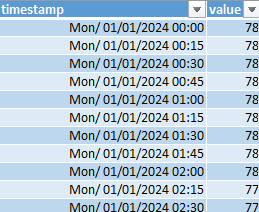
\includegraphics[width=0.4\textwidth]{Example_Excel.png}
    \caption{Example of a table}
    \label{fig:bild}
\end{figure}

Since B\'ezier interpolation is performed on
numerical variables, the timestamp column is first converted into a numerical
time scale. In the implementation, the first timestamp is used as the origin,
and all later timestamps are expressed as hours since this initial time.

\begin{lstlisting}[
    style=pythontextstyle,
    caption={Loading and preprocessing of the reference data.},
    label={lst:load-reference-data-python}
]
def load_reference_data(excel_path):
    df = pd.read_excel(excel_path)

    df = df[["timestamp", "value"]].dropna().copy()
    df["timestamp"] = pd.to_datetime(df["timestamp"])
    df = df.sort_values("timestamp").drop_duplicates(subset="timestamp")

    t0 = df["timestamp"].iloc[0]
    df["x_hours"] = (df["timestamp"] - t0).dt.total_seconds() / 3600.0

    return df["x_hours"].to_numpy(dtype=float), df["value"].to_numpy(dtype=float)
\end{lstlisting}

After the reference data have been loaded, support points are selected at a
prescribed step size. In the numerical experiments, the value
\(\texttt{step}=672\) was used, representing a week as a distance. The final data point is added
explicitly if it is not already included, so that the interpolation always
covers the full observation interval.

\begin{lstlisting}[
    style=pythontextstyle,
    caption={Selection of support points from the reference data.},
    label={lst:support-points-python}
]
def choose_support_points(x_ref, y_ref, step):
    idx = np.arange(0, len(x_ref), step)

    if idx[-1] != len(x_ref) - 1:
        idx = np.append(idx, len(x_ref) - 1)

    return idx, x_ref[idx], y_ref[idx]
\end{lstlisting}

Thus, the full reference data set is used for evaluation and comparison,
while the B\'ezier interpolants themselves are constructed only from the
selected support values.

\subsection{Computation of Empirical Interval Means}

For each interval between two consecutive support points, the prescribed mean
value is computed from the original reference data. Let \(a\) and \(b\) be
the indices of two neighboring support points. Then all measured values

\[
y_a^{\mathrm{ref}},y_{a+1}^{\mathrm{ref}},\dots,y_b^{\mathrm{ref}}
\]

are included in the empirical mean. In Python, the expression
\(\texttt{y\_ref[a:b+1]}\) is used because the upper bound of a Python slice is
not included.

\begin{lstlisting}[
    style=pythontextstyle,
    caption={Computation of empirical interval means from reference data.},
    label={lst:interval-means-python}
]
def compute_interval_means_from_reference(y_ref, idx):
    means = []

    for i in range(len(idx) - 1):
        a = idx[i]
        b = idx[i + 1]
        means.append(np.mean(y_ref[a:b + 1]))

    return np.asarray(means, dtype=float)
\end{lstlisting}

Mathematically, this corresponds to

\[
m_i =
\frac{1}{b-a+1}
\sum_{j=a}^{b} y_j^{\mathrm{ref}}.
\]

\subsection{Construction of the Mean-Preserving Cubic B\'ezier Method}

The cubic method constructs one cubic B\'ezier segment on each interval.
In the implementation, preferred values for \(P_1\) and \(P_2\) are first computed. If physical bounds are prescribed, this preferred pair is then projected onto the feasible interval defined by the exact mean constraint and the lower and upper bounds.

\begin{lstlisting}[
    style=pythontextstyle,
    caption={Construction of cubic B\'ezier control points with exact mean preservation.},
    label={lst:cubic-control-construction-python}
]
def _compute_bezier_control_points(
    y_nodes,
    means,
    lower_bound=None,
    upper_bound=None,
):
    n_intervals = len(y_nodes) - 1
    controls = np.zeros((n_intervals, 4), dtype=float)

    for i in range(n_intervals):
        y0 = y_nodes[i]
        y1 = y_nodes[i + 1]
        m = means[i]

        P0 = y0
        P3 = y1

        preferred_P1 = (2.0 / 3.0) * (y0 + y1) - 2.0 * m
        preferred_P2 = 6.0 * m - (5.0 / 3.0) * (y0 + y1)

        P1, P2 = _enforce_bounded_mean_pair(
            preferred_P1,
            preferred_P2,
            target_sum=4.0 * m - y0 - y1,
            lower_bound=lower_bound,
            upper_bound=upper_bound,
            interval_index=i,
        )

        controls[i] = [P0, P1, P2, P3]

    return controls
\end{lstlisting}

The auxiliary projection function keeps the exact mean condition unchanged.
The value of \(P_1\) is restricted to the feasible interval, and \(P_2\) is
then determined from the required sum.

\begin{lstlisting}[
    style=pythontextstyle,
    caption={Projection of the cubic internal control points onto the bounded mean-preserving feasible set.},
    label={lst:cubic-projection-python}
]
def _enforce_bounded_mean_pair(
    preferred_p1,
    preferred_p2,
    target_sum,
    lower_bound=None,
    upper_bound=None,
    interval_index=None,
):
    if lower_bound is None and upper_bound is None:
        return float(preferred_p1), float(preferred_p2)

    lower = -np.inf if lower_bound is None else float(lower_bound)
    upper = np.inf if upper_bound is None else float(upper_bound)

    feasible_low = max(lower, target_sum - upper)
    feasible_high = min(upper, target_sum - lower)

    if feasible_low > feasible_high:
        raise ValueError(
            "No feasible bounded B\'ezier segment for interval "
            f"{interval_index}: exact mean preservation conflicts "
            f"with the requested bounds."
        )

    projected_p1 = 0.5 * (preferred_p1 - preferred_p2 + target_sum)
    p1 = min(max(projected_p1, feasible_low), feasible_high)
    p2 = target_sum - p1

    return float(p1), float(p2)
\end{lstlisting}

Because a scalar B\'ezier curve remains inside the convex hull of its control
points, bounded control points are sufficient to guarantee that the whole
cubic segment remains within the same physical bounds.

\subsection{Construction of the Exact Quartic B\'ezier Method}

\begin{lstlisting}[
    style=pythontextstyle,
    caption={Exact quartic B\'ezier construction with endpoint, mean, and derivative constraints.},
    label={lst:exact-quartic-control-construction-python}
]
def _compute_quartic_bezier_control_points(
    x_nodes,
    y_nodes,
    means,
    derivatives,
    lower_bound,
    upper_bound,
    strict_bounds,
):
    n_intervals = len(x_nodes) - 1
    controls = np.zeros((n_intervals, 5), dtype=float)

    for i in range(n_intervals):
        h = x_nodes[i + 1] - x_nodes[i]

        y0 = y_nodes[i]
        y1 = y_nodes[i + 1]
        m = means[i]

        d0 = derivatives[i]
        d1 = derivatives[i + 1]

        P0 = y0
        P1 = y0 + (h / 4.0) * d0
        P3 = y1 - (h / 4.0) * d1
        P4 = y1
        P2 = 5.0 * m - P0 - P1 - P3 - P4

        segment_controls = np.array([P0, P1, P2, P3, P4], dtype=float)

        if strict_bounds:
            _check_bounds_for_control_points(
                segment_controls,
                interval_index=i,
                lower_bound=lower_bound,
                upper_bound=upper_bound,
            )

        controls[i] = segment_controls

    return controls
\end{lstlisting}

This method is useful as a diagnostic reference because it shows what happens
when the derivative conditions are imposed exactly.

\subsection{Derivative Estimation}

The exact and bounded quartic methods require derivative information at the
support points. Since such derivatives are not directly measured, they are
estimated numerically from the support values. The implementation allows two
methods: ordinary finite differences and a PCHIP-like derivative estimate.
The PCHIP-like method is used as the default because it reduces the risk of
artificial oscillations.

\begin{lstlisting}[
    style=pythontextstyle,
    caption={Selection of the derivative estimation method.},
    label={lst:derivative-method-python}
]
def estimate_node_derivatives(x_nodes, y_nodes, method="pchip"):
    x_nodes, y_nodes = _validate_xy_nodes(x_nodes, y_nodes)

    if method == "pchip":
        return estimate_pchip_derivatives_numpy(x_nodes, y_nodes)

    if method == "finite_difference":
        return np.gradient(y_nodes, x_nodes)

    raise ValueError(
        "Unknown derivative_method. Use 'pchip' or 'finite_difference'."
    )
\end{lstlisting}

For an interior support point, the PCHIP-like method first computes the
neighboring secant slopes. If the signs of two neighboring slopes are
different, the derivative is set to zero. This prevents the construction from
introducing artificial extrema. If the slopes have the same sign, a weighted
harmonic mean is used.

\begin{lstlisting}[
    style=pythontextstyle,
    caption={Interior PCHIP-like derivative estimation.},
    label={lst:pchip-derivatives-python}
]
h = np.diff(x)
delta = np.diff(y) / h
d = np.zeros(n, dtype=float)

for i in range(1, n - 1):
    left = delta[i - 1]
    right = delta[i]

    if left == 0.0 or right == 0.0 or np.sign(left) != np.sign(right):
        d[i] = 0.0
    else:
        w1 = 2.0 * h[i] + h[i - 1]
        w2 = h[i] + 2.0 * h[i - 1]
        d[i] = (w1 + w2) / (w1 / left + w2 / right)
\end{lstlisting}

Thus, the derivative estimates are local and shape-preserving. In the exact
quartic method they are imposed as hard constraints, while in the bounded
quartic method they are only used as preferred reference slopes.

\subsection{Construction of the Bounded Quartic B\'ezier Method}

The bounded quartic method is the final constrained method. It keeps endpoint interpolation and mean preservation exact, but treats derivative information as soft. \(P_1\) and \(P_3\) are projected onto the
feasible set, and \(P_2\) is determined afterwards from the exact mean
condition, if they were incompatible with the
physical bounds.

\begin{lstlisting}[
    style=pythontextstyle,
    caption={Bounded quartic B\'ezier construction with soft derivative constraints.},
    label={lst:bounded-quartic-control-construction-python}
]
def _compute_bounded_quartic_control_points(
    x_nodes,
    y_nodes,
    means,
    derivatives,
    lower_bound,
    upper_bound,
):
    n_intervals = len(x_nodes) - 1
    controls = np.zeros((n_intervals, 5), dtype=float)

    for i in range(n_intervals):
        h = x_nodes[i + 1] - x_nodes[i]

        y0 = y_nodes[i]
        y1 = y_nodes[i + 1]
        m = means[i]

        d0 = derivatives[i]
        d1 = derivatives[i + 1]

        P0 = y0
        P4 = y1

        internal_sum = 5.0 * m - P0 - P4

        P1_ref = P0 + (h / 4.0) * d0
        P3_ref = P4 - (h / 4.0) * d1

        P1, P3 = _project_p1_p3_to_bounded_mean_feasible_set(
            target_p1=P1_ref,
            target_p3=P3_ref,
            internal_sum=internal_sum,
            lower_bound=lower_bound,
            upper_bound=upper_bound,
            interval_index=i,
        )

        P2 = internal_sum - P1 - P3

        segment_controls = np.array([P0, P1, P2, P3, P4], dtype=float)

        _check_bounds_for_control_points(
            segment_controls,
            interval_index=i,
            lower_bound=lower_bound,
            upper_bound=upper_bound,
        )

        controls[i] = segment_controls

    return controls
\end{lstlisting}

The projection problem is two-dimensional because \(P_2\) is determined by
the mean condition once \(P_1\) and \(P_3\) are known. The feasible set is
described by

\[
L\leq P_1\leq U,\qquad
L\leq P_3\leq U,\qquad
L\leq S_i-P_1-P_3\leq U,
\]

where

\[
S_i=5m_i-P_0-P_4.
\]

The implementation first checks whether such a feasible pair can exist.

\begin{lstlisting}[
    style=pythontextstyle,
    caption={Feasibility check for the bounded quartic projection problem.},
    label={lst:bounded-quartic-feasibility-python}
]
lb = -np.inf if lower_bound is None else float(lower_bound)
ub = np.inf if upper_bound is None else float(upper_bound)

sum_low = -np.inf if upper_bound is None else internal_sum - ub
sum_high = np.inf if lower_bound is None else internal_sum - lb

min_possible_sum = 2.0 * lb
max_possible_sum = 2.0 * ub

feasible_sum_low = max(sum_low, min_possible_sum)
feasible_sum_high = min(sum_high, max_possible_sum)

if feasible_sum_low > feasible_sum_high:
    raise ValueError(
        f"Infeasible bounded quartic B\'ezier segment on interval {interval_index}: "
        f"endpoint values, exact mean and bounds cannot be satisfied simultaneously."
    )
\end{lstlisting}

After feasibility has been checked, candidates are generated from the
reference point itself and from the boundary lines of the feasible set. The
candidate with the smallest Euclidean distance to
\((P_1^{\mathrm{ref}},P_3^{\mathrm{ref}})\) is selected.

\begin{lstlisting}[
    style=pythontextstyle,
    caption={Selection of the closest feasible pair of internal quartic control points.},
    label={lst:bounded-quartic-candidate-python}
]
def add_candidate(p1, p3):
    p1 = float(p1)
    p3 = float(p3)

    if is_feasible(p1, p3):
        dist = (p1 - a) ** 2 + (p3 - b) ** 2
        candidates.append((dist, p1, p3))

add_candidate(a, b)

# Additional candidates are generated on the boundary lines
# P1 = lower/upper, P3 = lower/upper, and P1 + P3 = constant.

candidates.sort(key=lambda item: item[0])
_, best_p1, best_p3 = candidates[0]

return best_p1, best_p3
\end{lstlisting}

This construction preserves the endpoint values and interval means exactly.
It also enforces the physical bounds whenever the bounded problem is feasible.
The derivative information is retained as closely as possible, but it is not
allowed to destroy physical admissibility.

\subsection{Evaluation of the Piecewise B\'ezier Curves}

After the control points have been computed, each B\'ezier curve is evaluated
on a dense grid. The evaluation is performed locally on every support
interval. For this purpose, each physical interval \([x_i,x_{i+1}]\) is
mapped to the normalized local parameter interval \([0,1]\).

In the implementation, the normalized parameter values are generated by
\(\texttt{np.linspace}\). They are then mapped back to the original time
scale by

\[
x=x_i+(x_{i+1}-x_i)t.
\]

\begin{lstlisting}[
    style=pythontextstyle,
    caption={Evaluation of a piecewise B\'ezier curve on a normalized local grid.},
    label={lst:evaluation-normalized-grid-python}
]
for i in range(len(x_nodes) - 1):
    x0 = x_nodes[i]
    x1 = x_nodes[i + 1]

    if i < len(x_nodes) - 2:
        t = np.linspace(0.0, 1.0, num_points, endpoint=False)
    else:
        t = np.linspace(0.0, 1.0, num_points)

    x = x0 + (x1 - x0) * t
    y = evaluate_quartic_bezier_segment(controls[i], t)

    x_all.append(x)
    y_all.append(y)
\end{lstlisting}

The option \(\texttt{endpoint=False}\) is used on all intervals except the
last one. This avoids duplicating support points at interval boundaries. The
last interval includes its right endpoint, so the final support point is
included in the evaluated curve.

When the curve is evaluated at a specific point \(x\), the same normalization
is used explicitly:

\[
t=\frac{x-x_i}{x_{i+1}-x_i}.
\]

This is also the normalization used in the Excel/VBA implementation.

\subsection{Verification of Constraints}

After construction and evaluation, the methods are checked numerically. The
verification step is important because the formulas impose the constraints
analytically, but the implementation must still be checked for numerical
errors and possible bound violations.

For the cubic method, the verification routine checks endpoint interpolation
and mean preservation. The maximum point error and maximum mean error are
stored over all intervals.

\begin{lstlisting}[
    style=pythontextstyle,
    caption={Verification of endpoint and mean preservation for the cubic method.},
    label={lst:cubic-verification-python}
]
err_left = abs(P[0] - y_nodes[i])
err_right = abs(P[3] - y_nodes[i + 1])

mean_val = np.sum(P) / 4.0
err_mean = abs(mean_val - means[i])

max_point_error = max(max_point_error, err_left, err_right)
max_mean_error = max(max_mean_error, err_mean)
\end{lstlisting}

For the exact quartic method, endpoint values, interval means, endpoint
derivatives, and physical bounds are checked. The derivative errors are
computed from the endpoint derivative formulas.

\begin{lstlisting}[
    style=pythontextstyle,
    caption={Verification of mean and derivative constraints for the exact quartic method.},
    label={lst:exact-quartic-verification-python}
]
mean_value = np.mean(P)
max_mean_error = max(max_mean_error, abs(mean_value - means[i]))

left_derivative = 4.0 * (P[1] - P[0]) / h
right_derivative = 4.0 * (P[4] - P[3]) / h

max_derivative_error = max(
    max_derivative_error,
    abs(left_derivative - derivatives[i]),
    abs(right_derivative - derivatives[i + 1]),
)
\end{lstlisting}

For the bounded quartic method, the derivatives are not hard constraints.
Therefore, the verification routine reports the maximum derivative change
instead of a derivative violation. This quantity measures how much the final
curve had to deviate from the preferred derivative values in order to satisfy
the mean and bound constraints.

\begin{lstlisting}[
    style=pythontextstyle,
    caption={Diagnostic derivative change for the bounded quartic method.},
    label={lst:bounded-quartic-derivative-change-python}
]
actual_left_derivative = 4.0 * (P[1] - P[0]) / h
actual_right_derivative = 4.0 * (P[4] - P[3]) / h

max_derivative_change = max(
    max_derivative_change,
    abs(actual_left_derivative - preferred_derivatives[i]),
    abs(actual_right_derivative - preferred_derivatives[i + 1]),
)
\end{lstlisting}

Physical bounds are checked directly on the control points. This is sufficient
because the scalar B\'ezier curve lies inside the convex hull of its control
points.

\begin{lstlisting}[
    style=pythontextstyle,
    caption={Verification of lower and upper bound violations.},
    label={lst:bound-verification-python}
]
if lower_bound is None:
    max_lower_violation = 0.0
else:
    max_lower_violation = float(
        np.max(np.maximum(lower_bound - controls, 0.0))
    )

if upper_bound is None:
    max_upper_violation = 0.0
else:
    max_upper_violation = float(
        np.max(np.maximum(controls - upper_bound, 0.0)))
\end{lstlisting}

The resulting verification report contains the maximum endpoint error, the
maximum mean error, derivative error or derivative change, and possible lower
or upper bound violations.

\subsection{Error Analysis and Numerical Comparison}

The interpolation methods are compared by evaluating their curves on a dense
grid and comparing these values with the reference data. Since the reference
measurements are available only at discrete timestamps, the reference values
on the dense grid are obtained by linear interpolation.

\begin{lstlisting}[
    style=pythontextstyle,
    caption={Evaluation of reference values on the dense comparison grid.},
    label={lst:reference-values-python}
]
x_plot, y_plot = evaluate_bounded_quartic_bezier(
    x_nodes=x_nodes,
    controls=controls,
    num_points=num_points,
)

y_true = np.interp(x_plot, x_ref, y_ref)
\end{lstlisting}

The residuals are defined as the difference between the reference values and
the B\'ezier approximation. From these residuals, the script computes the
root-mean-square error, mean absolute error, maximum absolute error, and the
coefficient of determination.

\begin{lstlisting}[
    style=pythontextstyle,
    caption={Computation of approximation error metrics.},
    label={lst:error-metrics-python}
]
def compute_error_metrics(y_true, y_pred):
    residuals = y_true - y_pred

    rmse = float(np.sqrt(np.mean(residuals ** 2)))
    mae = float(np.mean(np.abs(residuals)))
    max_abs_error = float(np.max(np.abs(residuals)))

    ss_res = float(np.sum(residuals ** 2))
    ss_tot = float(np.sum((y_true - np.mean(y_true)) ** 2))
    r2 = np.nan if ss_tot == 0 else float(1.0 - ss_res / ss_tot)

    return {
        "RMSE": rmse,
        "MAE": mae,
        "MAX": max_abs_error,
        "R2": r2,
        "residuals": residuals,
    }
\end{lstlisting}

For each method, the evaluated curve, the computed error metrics, the
constraint report, and the control points are stored in a dictionary. This
makes it possible to print tables, plot all methods together, and compare the
diagnostic quantities in a uniform way.

\begin{lstlisting}[
    style=pythontextstyle,
    caption={Storage of method results for comparison.},
    label={lst:method-result-dictionary-python}
]
results[name] = {
    "x": x_plot,
    "y": y_plot,
    "metrics": compute_error_metrics(y_true, y_plot),
    "constraints": constraints,
    "controls": controls,
}
\end{lstlisting}

The comparison script applies this structure to three methods: the
mean-preserving cubic B\'ezier method, the exact quartic B\'ezier method used
as a diagnostic reference, and the bounded quartic B\'ezier method with soft
derivative constraints.

\subsection{Control-Polygon Roughness}

In addition to the standard approximation errors, the bounded quartic method
also computes the roughness of the control polygon. This quantity is not an
interpolation constraint. It is only used as a diagnostic indicator of local
bending or possible oscillatory behavior.

\begin{lstlisting}[
    style=pythontextstyle,
    caption={Computation of the control-polygon roughness.},
    label={lst:roughness-python}
]
def compute_control_polygon_roughness(controls):
    controls = np.asarray(controls, dtype=float)
    roughness = 0.0

    for P in controls:
        second_diff = P[:-2] - 2.0 * P[1:-1] + P[2:]
        roughness += float(np.sum(second_diff ** 2))

    return roughness
\end{lstlisting}

A larger roughness value indicates stronger variation in the control polygon.
This can be useful when two methods have similar approximation errors but one
of them produces a visibly less regular curve.

\subsection{Graphical Diagnostics}

The numerical comparison is complemented by graphical diagnostics. The first
plot shows the reference data, the selected support points, and the B\'ezier
curves. The second plot shows the residuals of the methods. This makes it
possible to inspect not only the size of the error, but also where the errors
occur.

\begin{lstlisting}[
    style=pythontextstyle,
    caption={Graphical comparison of the interpolation methods.},
    label={lst:plot-comparison-python}
]
def plot_comparison(x_ref, y_ref, x_nodes, y_nodes, results):
    plt.figure(figsize=(14, 7))
    plt.plot(x_ref, y_ref, label="Reference data", linewidth=1.3, alpha=0.75)

    for name, info in results.items():
        if "error" in info:
            continue

        plt.plot(info["x"], info["y"], label=name, linewidth=2.0)

    plt.scatter(x_nodes, y_nodes, label="Support points", s=25, zorder=3)

    plt.xlabel("Time since start [hours]")
    plt.ylabel("Value")
    plt.title("Cubic mean B\'ezier vs quartic B\'ezier variants")
    plt.grid(True, alpha=0.3)
    plt.legend()
    plt.tight_layout()
\end{lstlisting}

The residual plot is especially useful for detecting systematic deviations.
If the residuals are concentrated in specific intervals, this may indicate
that the selected support step is too large or that the local dynamics are
too complex for the chosen segment.

\subsection{Excel/VBA Implementation}

After the Python implementation had been tested, the bounded quartic B\'ezier method was translated into Excel/VBA. The purpose of this step was practical: hydrological and hydrochemical data are often stored and inspected in Excel, so the final method should be usable directly in a spreadsheet environment.

The VBA implementation follows the same main steps as the Python version. It reads the original data from columns A and B, builds support points, computes empirical interval means, checks feasibility, constructs bounded quartic B\'ezier control points, evaluates the interpolated curve, writes the results back to the worksheet.

\begin{figure}[H]
    \hspace{-3.5cm}
    \includegraphics[width=1.5\textwidth]{VBA_Table_Result_Example.png}
    \caption{Example of a final table}
    \label{fig:bild}
\end{figure}

Then it creates a comparison chart for visualization of the interpolation results.

\begin{figure}[H]
    \hspace{-3.25cm}
    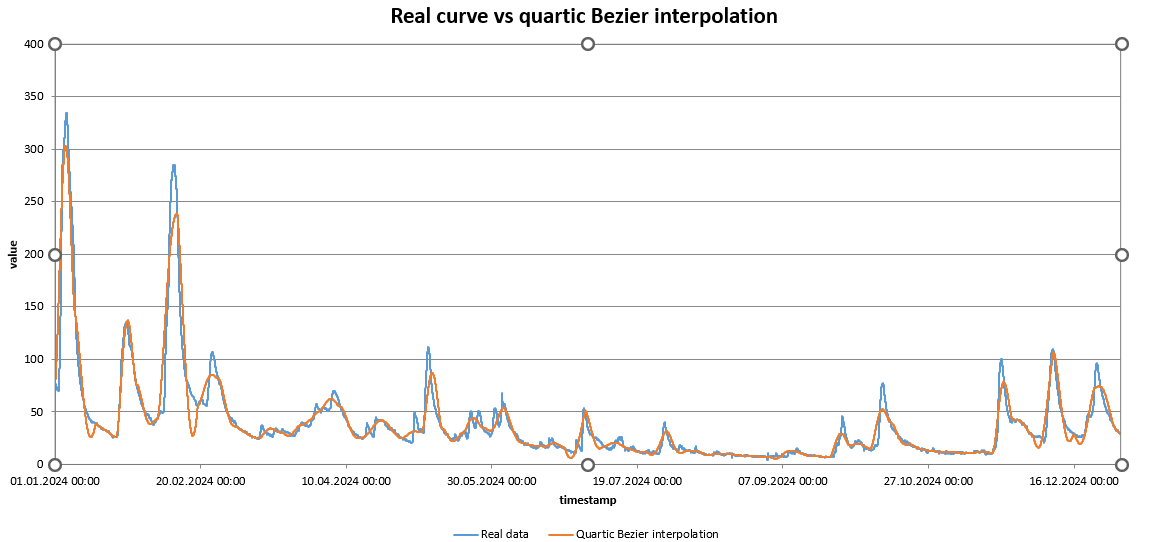
\includegraphics[width=1.5\textwidth]{Chart.png}
    \caption{Interpolated curve compared with measured data.}
    \label{fig:chart}
\end{figure}

The data input stage reads the original timestamps and values from the
worksheet and stores them in arrays.

\begin{lstlisting}[
    style=vbatextstyle,
    caption={Reading original data from the Excel worksheet.},
    label={lst:vba-read-data}
]
Dim rawX() As Double
Dim rawY() As Double
ReDim rawX(0 To nRaw - 1)
ReDim rawY(0 To nRaw - 1)

For i = 0 To nRaw - 1

    If IsEmpty(ws.Cells(DATA_FIRST_ROW + i, COL_X).Value) Or _
       IsEmpty(ws.Cells(DATA_FIRST_ROW + i, COL_Y).Value) Then
        MsgBox "Empty cell found in row " & (DATA_FIRST_ROW + i) & ".", vbCritical
        Exit Sub
    End If
    rawX(i) = CDbl(ws.Cells(DATA_FIRST_ROW + i, COL_X).Value)
    rawY(i) = CDbl(ws.Cells(DATA_FIRST_ROW + i, COL_Y).Value)
    
Next i
\end{lstlisting}

Support indices are then created using the prescribed value
\(\texttt{SUPPORT\_STEP}\). As in Python, the last data point is added if it
is not already part of the support set.

\begin{lstlisting}[
    style=vbatextstyle,
    caption={Construction of support point indices in VBA.},
    label={lst:vba-support-indices}
]
For i = 0 To nRaw - 1 Step SUPPORT_STEP
    supportCount = supportCount + 1
Next i

If (nRaw - 1) Mod SUPPORT_STEP <> 0 Then
    supportCount = supportCount + 1
End If

ReDim supportIndex(0 To supportCount - 1)

k = 0

For i = 0 To nRaw - 1 Step SUPPORT_STEP
    supportIndex(k) = i
    k = k + 1
Next i

If supportIndex(k - 1) <> nRaw - 1 Then
    supportIndex(k) = nRaw - 1
End If
\end{lstlisting}

The empirical means are computed in the same way as in Python: all original
values between two consecutive support indices are summed and divided by
their number.

\begin{lstlisting}[
    style=vbatextstyle,
    caption={Computation of empirical interval means in VBA.},
    label={lst:vba-interval-means}
]
For i = 0 To supportCount - 2

    startIdx = supportIndex(i)
    endIdx = supportIndex(i + 1)

    sumY = 0#
    countY = 0

    For j = startIdx To endIdx
        sumY = sumY + rawY(j)
        countY = countY + 1
    Next j

    means(i) = sumY / countY

Next i
\end{lstlisting}

Before constructing the bounded quartic curve, the VBA implementation checks
whether the exact mean and lower bound are compatible. In the case
\(L=0\), a necessary feasibility condition is

\[
m_i \geq \frac{y_i+y_{i+1}}{5}.
\]

\begin{lstlisting}[
    style=vbatextstyle,
    caption={Feasibility check for the bounded quartic construction in VBA.},
    label={lst:vba-feasibility-check}
]
For i = 0 To supportCount - 2

    minimalMean = (yNodes(i) + yNodes(i + 1)) / 5#

    If means(i) < minimalMean Then
        MsgBox _
            "Problem on interval " & i & vbCrLf & _
            "true interval mean = " & means(i) & vbCrLf & _
            "minimal possible mean with lower bound 0 = " & minimalMean & vbCrLf & _
            "This interval is infeasible.", _
            vbCritical
        Exit Sub
    End If

Next i
\end{lstlisting}

The bounded quartic control points are then constructed by the VBA function
\(\texttt{BuildBoundedQuarticBezierControls}\), which internally estimates
PCHIP-like derivatives and applies the same bounded quartic projection logic
as the Python version.

\begin{lstlisting}[
    style=vbatextstyle,
    caption={Calling the bounded quartic B\'ezier construction in VBA.},
    label={lst:vba-build-controls}
]
controls = BuildBoundedQuarticBezierControls( _
    xNodes, _
    yNodes, _
    means, _
    LOWER_BOUND, _
    USE_UPPER_BOUND, _
    UPPER_BOUND _
)
\end{lstlisting}

For the evaluation at a given worksheet timestamp, the corresponding interval
is found and the local normalized parameter \(t\) is computed as

\[
t=\frac{x-x_i}{x_{i+1}-x_i}.
\]

\begin{lstlisting}[
    style=vbatextstyle,
    caption={Evaluation of the piecewise quartic B\'ezier curve at a worksheet timestamp.},
    label={lst:vba-evaluate-at-x}
]
If xValue >= xNodes(i) And xValue <= xNodes(i + 1) Then

    t = (xValue - xNodes(i)) / (xNodes(i + 1) - xNodes(i))

    EvaluatePiecewiseQuarticBezierAtX = EvaluateQuarticBezierSegment( _
        controls(i, 0), controls(i, 1), controls(i, 2), _
        controls(i, 3), controls(i, 4), t _
    )

    Exit Function

End If
\end{lstlisting}

The computed support intervals, control points, evaluated interpolation, and
verification values are written back into the worksheet. The main worksheet
layout is summarized in Table~\ref{tab:vba-output-ranges}.

\begin{table}[H]
\centering
\begin{tabular}{ll}
\toprule
Worksheet range & Content \\
\midrule
A:B & Original timestamps and measured values \\
D:M & Support intervals and B\'ezier control points \\
O:Q & Original values and evaluated interpolation \\
S:T & Verification quantities \\
Chart area & Visual comparison of measured data and interpolation \\
\bottomrule
\end{tabular}
\caption{Main worksheet input and output ranges used by the Excel/VBA implementation.}
\label{tab:vba-output-ranges}
\end{table}

The VBA implementation is therefore not a separate mathematical method. It is
an operational translation of the bounded quartic B\'ezier construction into
Excel.

\subsection{Summary of the Implementation Logic}

The complete implementation can be summarized as follows:

\begin{enumerate}
    \item The original measured data are loaded from Excel or from an Excel file.
    \item Timestamps are converted into a numerical time variable.
    \item Support points are selected using a fixed step size.
    \item Empirical interval means are computed from all original values inside each support interval.
    \item Cubic, exact quartic, and bounded quartic B\'ezier control points are constructed.
    \item The exact quartic method uses derivative estimates as hard constraints.
    \item The bounded quartic method uses derivative estimates only as soft reference slopes.
    \item Physical bounds are enforced through the B\'ezier control points.
    \item The piecewise curves are evaluated using the normalized local parameter \(t\in[0,1]\).
    \item Constraint errors, bound violations, derivative errors or derivative changes, and roughness values are computed.
    \item The approximations are compared with the original reference data using RMSE, MAE, maximum error, and \(R^2\).
    \item The curves and residuals are plotted for visual inspection.
\end{enumerate}

This organization separates the mathematical construction from the practical
workflow.

\subsection{Source Codes}

The complete Python and VBA source codes used for the implementation and
numerical comparison of the investigated methods are provided in the
Attachments. The mean-preserving cubic B\'ezier implementation is given in
Listing~\ref{lst:cubic-bezier-code}. The exact quartic B\'ezier
implementation is given in Listing~\ref{lst:quartic-bezier-code}. The
modified bounded quartic B\'ezier implementation with soft derivative
constraints is given in Listing~\ref{lst:bounded-quartic-bezier-code}. The
script used for numerical comparison is given in
Listing~\ref{lst:comparison-code}, and the Excel/VBA implementation is given
in Listing~\ref{lst:vba-bezier-code}.

\newpage
\section{Numerical Results and Comparison}

This section presents the numerical comparison of the three B\'ezier-based
interpolation methods considered in this work. The comparison is based on approximation accuracy, preservation
of the imposed constraints, physical admissibility, and visual behavior of the
final curves.

The results must be interpreted with respect to two different aspects. First,
the interpolating curve should approximate the reference data accurately.
Second, it must satisfy the prescribed mathematical and physical constraints.
Therefore, a method with good error metrics cannot be considered fully
satisfactory if it violates the physical bound or does not preserve the
interval means.

\subsection{Numerical Setup}

The numerical experiment was performed on a reference data set containing
35136 measured values. Support points were selected with a fixed step size of
672, resulting in 54 support points and 53 interpolation intervals. The
interval means were computed as sample averages of the original reference
values within each support interval. The lower physical bound was set to zero,
while no upper bound was imposed. For the quartic methods, the derivative
values were estimated using the PCHIP-like derivative estimator.

\begin{table}[H]
\centering
\begin{tabular}{lc}
\toprule
Quantity & Value \\
\midrule
Number of reference points & 35136 \\
Number of support points & 54 \\
Number of interpolation intervals & 53 \\
Support step size & 672 \\
Mean computation mode & Sample average \\
Lower physical bound & 0.0 \\
Upper physical bound & Not imposed \\
Quartic derivative method & PCHIP-like \\
\bottomrule
\end{tabular}
\caption{Numerical setup used for the comparison of the interpolation methods.}
\label{tab:numerical-setup}
\end{table}

This information is important for reproducibility, since the
number of support points, the support step size, and the imposed physical
bounds directly influence the interpolation result. In particular, the
support step size determines how much information is available to reconstruct
the behavior between two neighboring support points.

\subsection{Approximation Quality}

The first part of the comparison concerns approximation quality. Each
interpolating curve was evaluated on a dense grid and compared with the
reference data. The considered error metrics are the root-mean-square error
\(\mathrm{RMSE}\), the mean absolute error \(\mathrm{MAE}\), the maximum
absolute error, and the coefficient of determination \(R^2\). In addition,
the control-polygon roughness is reported as a diagnostic indicator of local
bending and possible oscillatory behavior.

\begin{table}[H]
\centering
\small
\resizebox{\textwidth}{!}{
\begin{tabular}{lrrrrr}
\toprule
Method & RMSE & MAE & Max. error & $R^2$ & Roughness \\
\midrule
Cubic B\'ezier baseline, mean-preserving
& 12.819150 & 7.452175 & 100.849592 & 0.910025 & $3.806379\times 10^{6}$ \\

Quartic B\'ezier, mean and hard derivatives
& 11.242047 & 5.560609 & 94.711293 & 0.930802 & $2.768685\times 10^{6}$ \\

Bounded quartic B\'ezier with soft derivatives
& 10.947902 & 5.470358 & 94.711293 & 0.934376 & $2.136015\times 10^{6}$ \\
\bottomrule
\end{tabular}
}
\caption{Approximation quality and control-polygon roughness of the considered B\'ezier interpolation methods.}
\label{tab:approximation-quality}
\end{table}

Table~\ref{tab:approximation-quality} is needed to quantify how closely each
method follows the reference data.

The exact quartic B\'ezier method improves  an RMSE, an MAE, and \(R^2\). This shows that the additional degree of freedom in the quartic formulation and the use of derivative
information improve the approximation quality.

The bounded quartic B\'ezier method with soft derivative constraints gives
the best overall approximation quality among the tested methods. It has the
lowest RMSE, the lowest MAE, and the largest value of \(R^2\). Compared with
the cubic baseline, the bounded quartic method reduces the RMSE by
approximately \(14.6\%\) and the MAE by approximately \(26.6\%\). The
coefficient of determination increases from \(0.910025\) to \(0.934376\).

The roughness values show a similar tendency. The cubic method has the largest
control-polygon roughness, \(3.806379\times 10^6\). The exact quartic method
reduces this value to \(2.768685\times 10^6\), while the bounded quartic
method gives the smallest roughness, \(2.136015\times 10^6\). Thus, the
bounded quartic method not only improves the approximation error but also
produces a less rough control structure.

The maximum absolute error is reduced when moving from the cubic method to
the quartic methods. However, the exact quartic and bounded quartic methods
have the same maximum error of \(94.711293\). This suggests that the largest
local deviation is caused by a difficult interval or a sharp local feature in
the data, which is not fully resolved by the selected support spacing.
Therefore, the maximum error should be interpreted together with the residual
plot rather than as the only criterion for method quality.

\subsection{Constraint Verification}

The second part of the comparison concerns the imposed constraints.

\begin{table}[H]
\centering
\small
\resizebox{\textwidth}{!}{
\begin{tabular}{lrrrrr}
\toprule
Method 
& Endpoint error 
& Mean error 
& Control lower violation
& Dense minimum
& Dense lower violation \\
\midrule
Cubic B\'ezier baseline
& $0$
& $0$
& $0$
& 4.825098
& $0$ \\

Quartic B\'ezier
& $0$
& $2.842171\times 10^{-14}$
& $1.131798\times 10^{2}$
& 2.709591
& $0$ \\

Bounded quartic B\'ezier
& $0$
& $2.842171\times 10^{-14}$
& $0$
& 5.605888
& $0$ \\
\bottomrule
\end{tabular}
}
\caption{Verification of endpoint interpolation, mean preservation, and lower-bound admissibility. The control lower violation is computed from the B\'ezier control points, while the dense lower violation is computed from the evaluated curve on the dense grid.}
\label{tab:constraint-verification}
\end{table}

Table~\ref{tab:constraint-verification} shows that all methods preserve the
endpoint values exactly. The endpoint error is zero for all three methods,
which is expected because the first and last control points of each B\'ezier
segment are chosen to be the corresponding support values.

The interval mean is also preserved up to numerical precision. For the cubic
method, the maximum mean error is zero in the reported output. For the
quartic methods, the maximum mean error is \(2.842171\times 10^{-14}\), which
is negligible and can be interpreted as floating-point round-off error.
Therefore, the mean-preserving condition is successfully enforced by all
three constructions.

The main difference between the methods appears in the lower-bound
verification. The exact quartic method has a control lower violation of
\(1.131798\times 10^2\). This means that at least one control point lies below
the prescribed lower bound. The evaluated dense grid still has a positive
minimum value, so the sampled curve does not become negative in this
experiment. However, the convex-hull guarantee is lost: bounded control
points are a sufficient condition for the full scalar B\'ezier curve to remain
bounded. If a control point violates the bound, this guarantee no longer
holds.

This violation is not accidental. In the exact quartic formulation, the
endpoint values, the interval mean, and both endpoint derivatives are imposed
as hard constraints. These five conditions uniquely determine the five
control points of the quartic B\'ezier segment. Consequently, there is no
remaining degree of freedom to adjust the control polygon if the resulting
control points violate the physical lower bound.

In contrast, the bounded quartic B\'ezier method avoids this issue. It
preserves endpoint values and interval means up to numerical precision and
has no control lower violation. This is achieved by treating the derivative
estimates as soft reference slopes. The derivative information is used to
define preferred control points, but these points are modified whenever
necessary to preserve the lower bound and the exact mean constraint.

\subsection{Derivative Information}

The exact and bounded quartic methods both use derivative information, but in
different ways. In the exact quartic method, the derivatives are imposed as
hard constraints. The maximum derivative error is

\[
1.249001\times 10^{-16},
\]

which is essentially zero. This confirms that the derivative constraints are
implemented correctly. However, the same exact enforcement is also the reason
why physical bounds may become impossible to satisfy.

In the bounded quartic method, the derivative estimates are not imposed
unconditionally. Instead, they are treated as preferred reference slopes. The
maximum derivative change is

\[
1.361424.
\]

This value should not be interpreted as an interpolation error. It measures
how much the final bounded curve had to deviate from the preferred derivative
information in order to preserve endpoint interpolation, exact interval means,
and physical admissibility. Thus, the bounded quartic method deliberately
sacrifices exact derivative matching when the derivative constraints conflict
with the physical lower bound.

\subsection{Graphical Comparison}

The numerical tables are complemented by graphical diagnostics. The first
graph compares the original reference data, the selected support points, and
the three B\'ezier interpolation methods. The second graph shows the residuals,
defined as

\[
\text{residual}
=
\text{reference value}
-
\text{approximated value}.
\]

Thus, a positive residual means that the interpolation underestimates the
reference data, while a negative residual means that it overestimates them.

\begin{figure}[H]
    \centering
    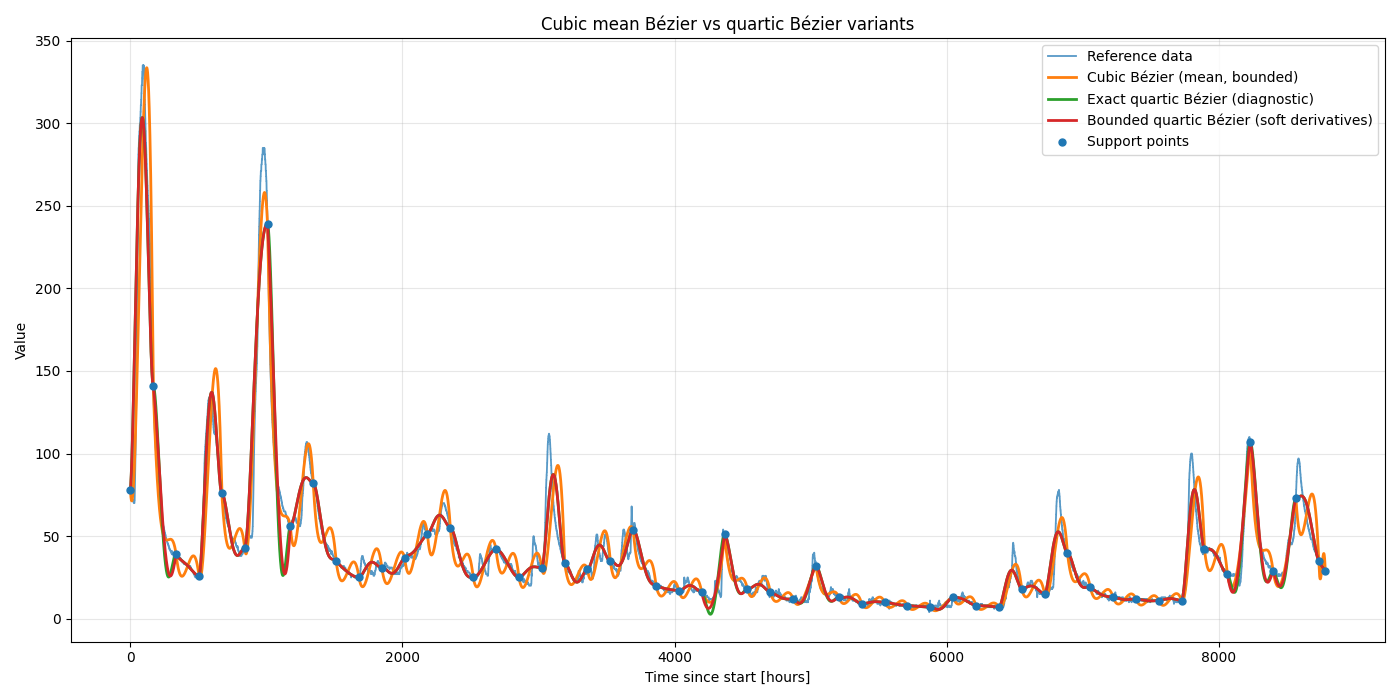
\includegraphics[width=1\textwidth]{Compare.png}
    \caption{Comparison of the reference data, support points, and the three B\'ezier interpolation methods.}
    \label{fig:method-comparison}
\end{figure}

Figure~\ref{fig:method-comparison} shows that all three methods reproduce the
general structure of the reference data. The largest difficulties occur near
sharp peaks and rapid transitions. This is expected, because the support
points are relatively sparse compared with the full reference data set, so
the interpolating curves must reconstruct local behavior over long support
intervals.

The cubic B\'ezier baseline follows the general trend, but it is less
flexible than the quartic methods. This is visible especially near larger
peaks, where the cubic curve cannot always reproduce the local shape as
closely. The exact quartic and bounded quartic methods generally follow the
reference data more accurately because they use derivative information and
have one additional control point.

However, the exact quartic method cannot be selected as the final method only
because it looks accurate. Table~\ref{tab:constraint-verification} shows that
it violates the lower-bound condition at the level of the control points.
Therefore, it does not provide the required convex-hull-based physical
guarantee. The bounded quartic method retains the improved flexibility of the
quartic formulation while correcting the internal control points whenever
necessary to preserve physical admissibility.

\begin{figure}[H]
    \centering
    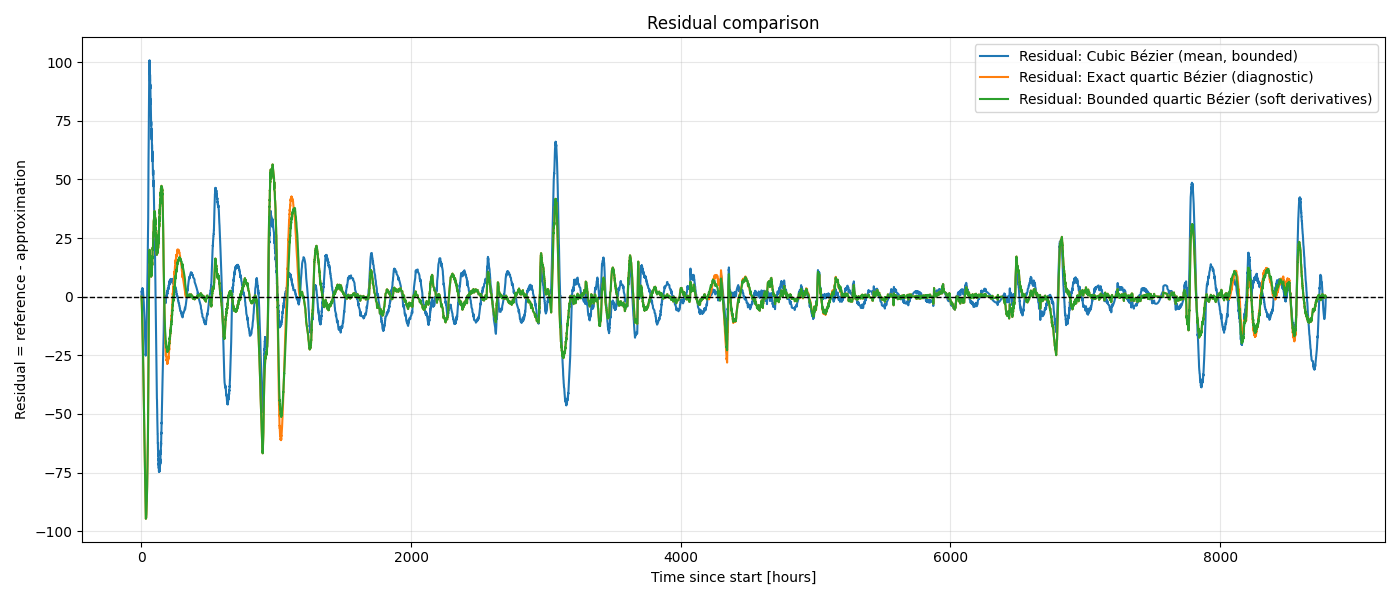
\includegraphics[width=1\textwidth]{Residual_comparison.png}
    \caption{Residual comparison of the three interpolation methods. The residual is defined as reference value minus approximated value.}
    \label{fig:residual-comparison}
\end{figure}

Figure~\ref{fig:residual-comparison} gives a more detailed view of the local
errors. The residuals are largest near sharp peaks and rapid changes,
especially in the first part of the time series. This explains why the
maximum absolute error remains relatively large even for the quartic methods.
The RMSE and MAE values show an overall improvement, but the largest local
deviations are concentrated in difficult intervals where the data change much
faster than the spacing of the support points.

The residuals of the bounded quartic method are generally smaller than those
of the cubic baseline, which is consistent with the lower RMSE and MAE values
in Table~\ref{tab:approximation-quality}. The residual behavior of the exact
quartic and bounded quartic methods is often similar, but the bounded method
has the additional advantage of satisfying the lower-bound condition through
bounded control points.

\subsection{Overall Interpretation}

The comparison shows that the bounded quartic B\'ezier method with soft
derivative constraints provides the best compromise among the three tested
methods. It achieves the best approximation quality according to RMSE, MAE,
and \(R^2\), reduces the control-polygon roughness compared with the cubic and
exact quartic methods, preserves endpoint values and interval means up to
numerical precision, and satisfies the lower-bound constraint.

The cubic B\'ezier baseline is stable and physically admissible, but it is
less accurate and less flexible. The exact quartic method improves the
approximation quality and satisfies the derivative constraints almost exactly,
but it violates the lower-bound condition at the level of the control points.
The bounded quartic method combines the advantages of the quartic formulation
with physical admissibility by treating derivative information as soft rather
than mandatory.

Therefore, the bounded quartic B\'ezier method is the most suitable method for
the present application. It preserves the essential mathematical constraints,
uses derivative information when it is compatible with the physical bound, and
modifies it only when necessary to maintain admissibility.

\newpage
\section{Conclusion}
This work investigated B\'ezier-based interpolation methods for the
approximation of hydrochemical and hydrological time-series data under
simultaneous mathematical and physical constraints. 

The main objective was not only to construct a smooth interpolating curve,
but also to preserve important properties of the original data.

Three B\'ezier-based methods were developed and compared. The first method
was a mean-preserving cubic B\'ezier construction. This method satisfied the
endpoint and mean constraints and remained physically admissible, but it had
less flexibility in representing local changes of the data. The second method
was an exact quartic B\'ezier formulation in which endpoint values, interval
means, and endpoint derivatives were imposed as hard constraints. This method
improved the approximation quality, but it also demonstrated an important
limitation: once all five quartic control points are fixed by these
constraints, there is no remaining freedom to enforce physical bounds. As a
result, the exact quartic method may violate the lower-bound condition at the
level of the control points.

The final method was a bounded quartic B\'ezier formulation with soft
derivative constraints. In this method, derivative estimates are used as
reference slopes rather than mandatory constraints. The endpoint values and
interval means are preserved exactly, while the internal control points are
projected onto a feasible set whenever the derivative-based construction
would violate the prescribed physical bounds. This makes it possible to keep
the advantages of derivative-based quartic interpolation while maintaining
physical admissibility.

The numerical comparison showed that the bounded quartic B\'ezier method
provided the best compromise among the tested methods. It achieved the lowest
RMSE and MAE values and the highest coefficient of determination \(R^2\). It
also reduced the control-polygon roughness compared with the cubic and exact
quartic constructions. At the same time, it preserved endpoint values and
interval means up to numerical precision and avoided the lower-bound
violation observed in the exact quartic diagnostic method. Thus, the bounded
quartic formulation was the most suitable method for the present application.

The graphical comparison and residual analysis confirmed the quantitative
results. All methods captured the general structure of the measured time
series, but the largest errors occurred near sharp peaks and rapid
transitions. This is expected because the support points were relatively
sparse compared with the full reference data set. The quartic methods were
better able to represent the local shape of the data than the cubic method,
while the bounded quartic method additionally preserved the required physical
constraints.

The methods have implementations and tests in Python. The final bounded quartic method
was then translated into Excel/VBA. This second implementation makes the
method usable in a spreadsheet-based workflow.

Several limitations remain. The quality of the interpolation depends on the
choice of support points and on the reliability of the derivative estimates.
If the support points are too far apart, sharp peaks or rapid local changes
may not be reconstructed accurately. Furthermore, in this work the prescribed
interval means were computed as arithmetic averages of the measured values.
For data with irregular time spacing, a time-weighted mean could be more
appropriate. Finally, only a lower physical bound was considered in the
numerical experiments, while future applications may require both lower and
upper bounds.

Future work could therefore focus on adaptive support point selection,
improved derivative estimation, time-weighted mean preservation, automatic
detection of difficult intervals, and extension of the bounded construction
to more general physical constraints. Nevertheless, the results of this research
show that the bounded quartic B\'ezier method with soft derivative constraints
is a promising approach for physically consistent and mean-preserving
interpolation of sparse experimental time-series data.

% ------------------------------------------------------------
% Bibliography
% ------------------------------------------------------------
\clearpage
\printbibliography[heading=bibintoc,title={References}]

\clearpage
\phantomsection
\addcontentsline{toc}{section}{List of Figures}
\listoffigures

\clearpage
\phantomsection
\addcontentsline{toc}{section}{List of Tables}
\listoftables

\clearpage
\phantomsection
\addcontentsline{toc}{section}{List of Code Listings}
\lstlistoflistings
% ------------------------------------------------------------

\end{document}